\documentclass[First Project.tex]{subfiles}
\begin{document}

\subsection{ Σύγκριση επαναλήψεων για κάθε ρίζα }
Σε αυτή την παράγραφο γίνεται μία σύγκριση των επαναλήψεων που χρειάστηκε κάθε μέθοδος για την εύρεση των
τριών ριζών. Για  να είναι τα αποτελέσματα της σύγκρισης αυτής πιο αντιπροσωπευτικά χρησιμοποιήθηκε δείγμα 10000 κλήσεων των συναρτήσεων που υλοποιούν την κάθε μέθοδο
σε κατάλληλα διαστήματα και αρχικά σημεία και όχι τα μεμονωμένα ορίσματα που χρησιμοποιηθήκαν στις παραγράφους 2.1, 2.2 και 2.3. Εφόσον για την ρίζα \textlatin{\textbf{$x$= 0}} δεν μπορούν να βρεθούν κατάλληλα διαστήματα
και αρχικά σημεία έτσι ώστε να τηρούνται οι προϋποθέσεις για κάθε μέθοδο, η ρίζα αυτή δεν συμπεριλαμβάνεται σε αυτή την ανάλυση.
\subsubsection{\textbf{Μέθοδος της διχοτόμησης}}
\vspace{5mm}
\begin{figure}[h!]
    \centering
    \subfloat{{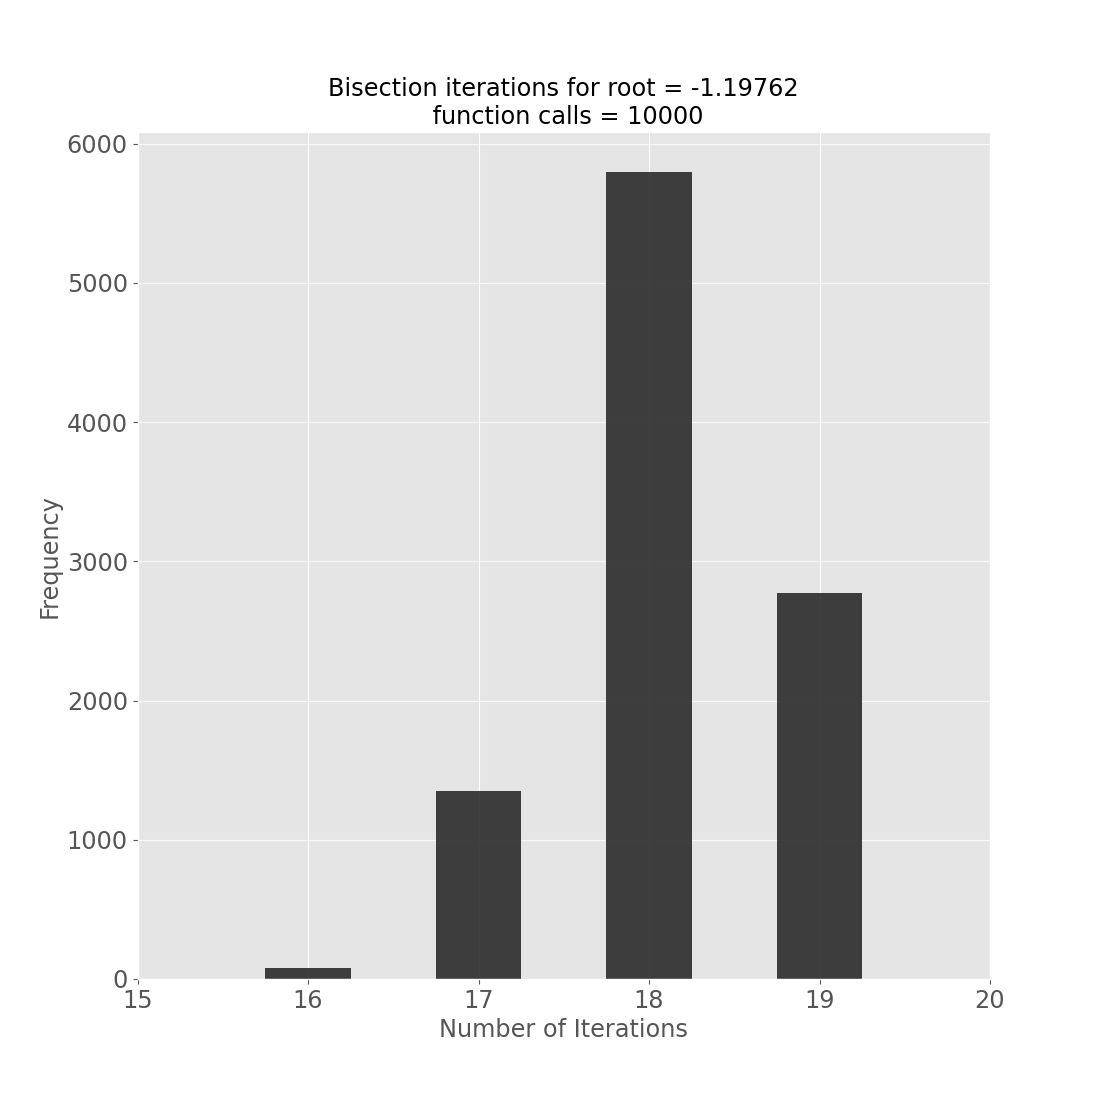
\includegraphics[scale=0.19]{bisection_iterations_first_root.png} }}
    \quad
    \subfloat{{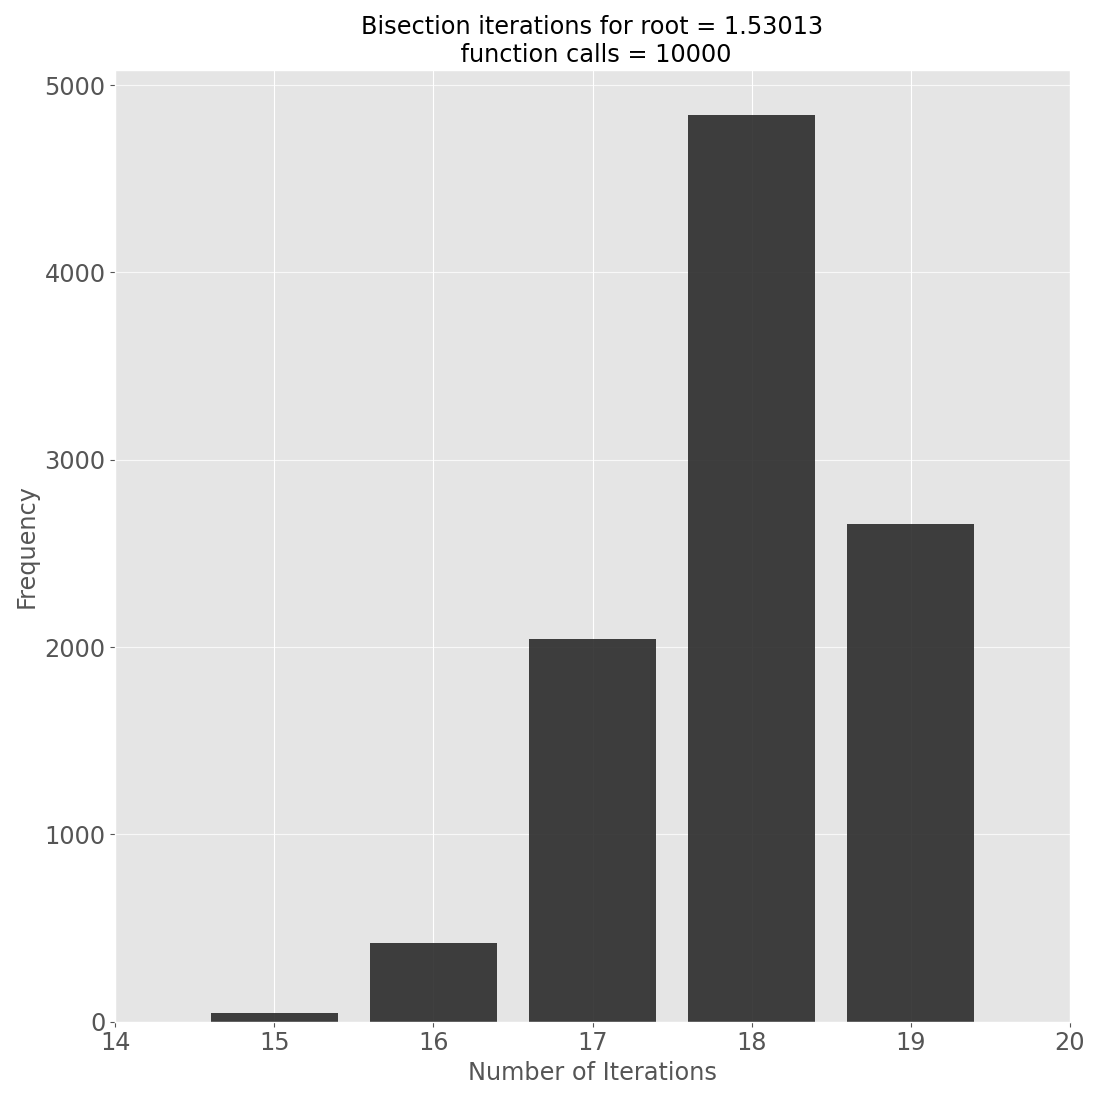
\includegraphics[scale=0.19]{bisection_iterations_third_root.png} }}
    \caption{ Ιστογράμματα συχνοτήτων του αριθμού των επαναλήψεων για την μέθοδο της διχοτόμησης. }
\end{figure}
Όπως παρατηρούμε από τα ιστογράμματα στο \textit{Σχήμα 24} η μέθοδος της διχοτόμησης αποδίδει σε αριθμούς επαναλήψεων γύρω από το 18.
\subsubsection{\textbf{Μέθοδος \textlatin{Newton-Raphson}}}
\vspace{5mm}
\begin{figure}[h!]
    \centering
    \subfloat{{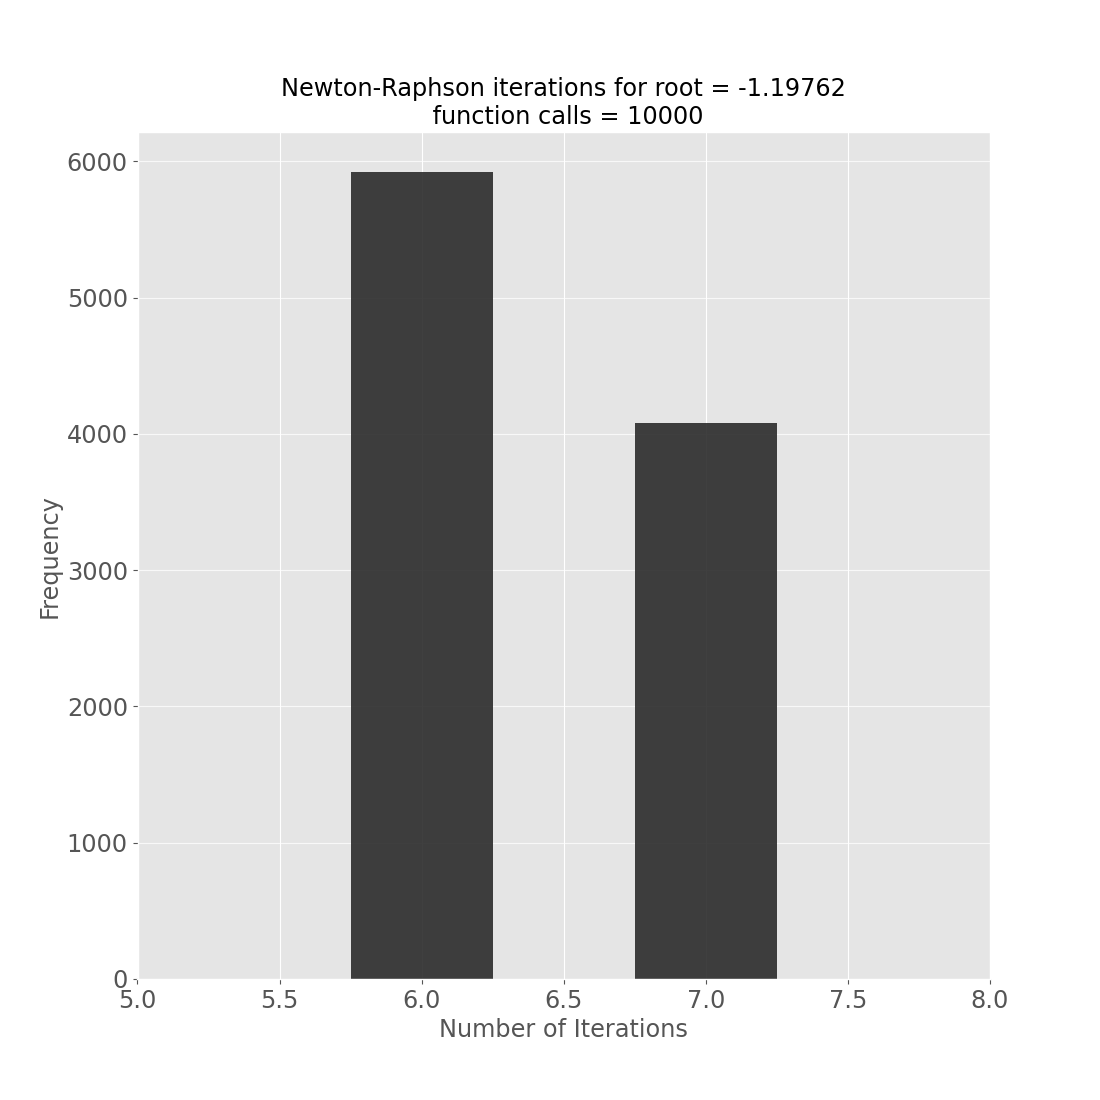
\includegraphics[scale=0.19]{newton_iterations_first_root.png} }}
    \quad
    \subfloat{{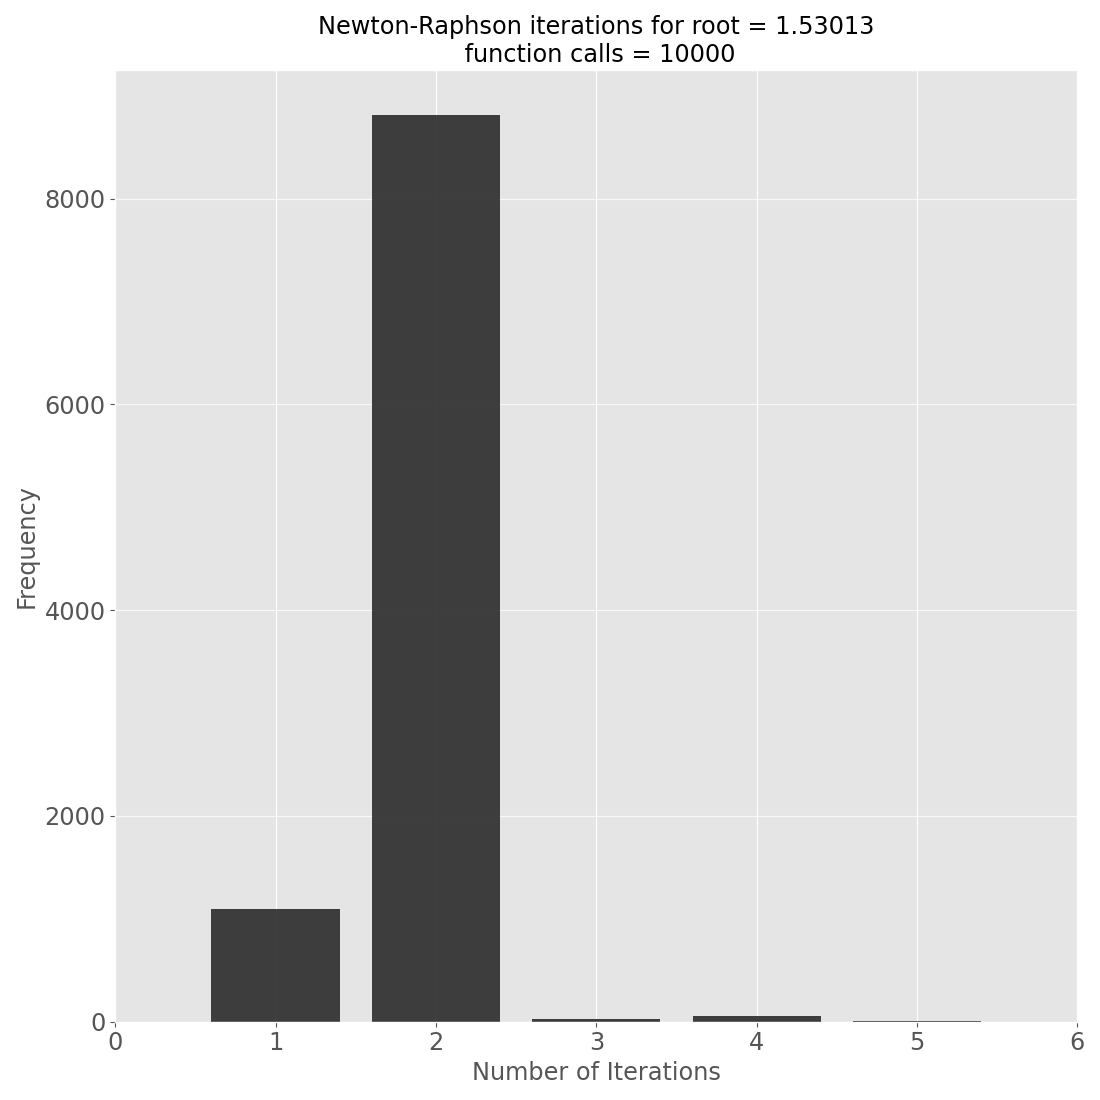
\includegraphics[scale=0.19]{newton_iterations_third_root.png} }}
    \caption{ Ιστογράμματα συχνοτήτων του αριθμού των επαναλήψεων για την μέθοδο \textlatin{Newton-Raphson}. }
\end{figure}
Όπως παρατηρούμε από τα ιστογράμματα στο \textit{Σχήμα 25} η μέθοδος \textlatin{Newton-Raphson} αποδίδει κυρίως σε 2,6 και
7 αριθμούς επαναλήψεων.
\newpage
\subsubsection{\textbf{Μέθοδος της τέμνουσας}}
\begin{figure}[h!]
    \centering
    \subfloat{{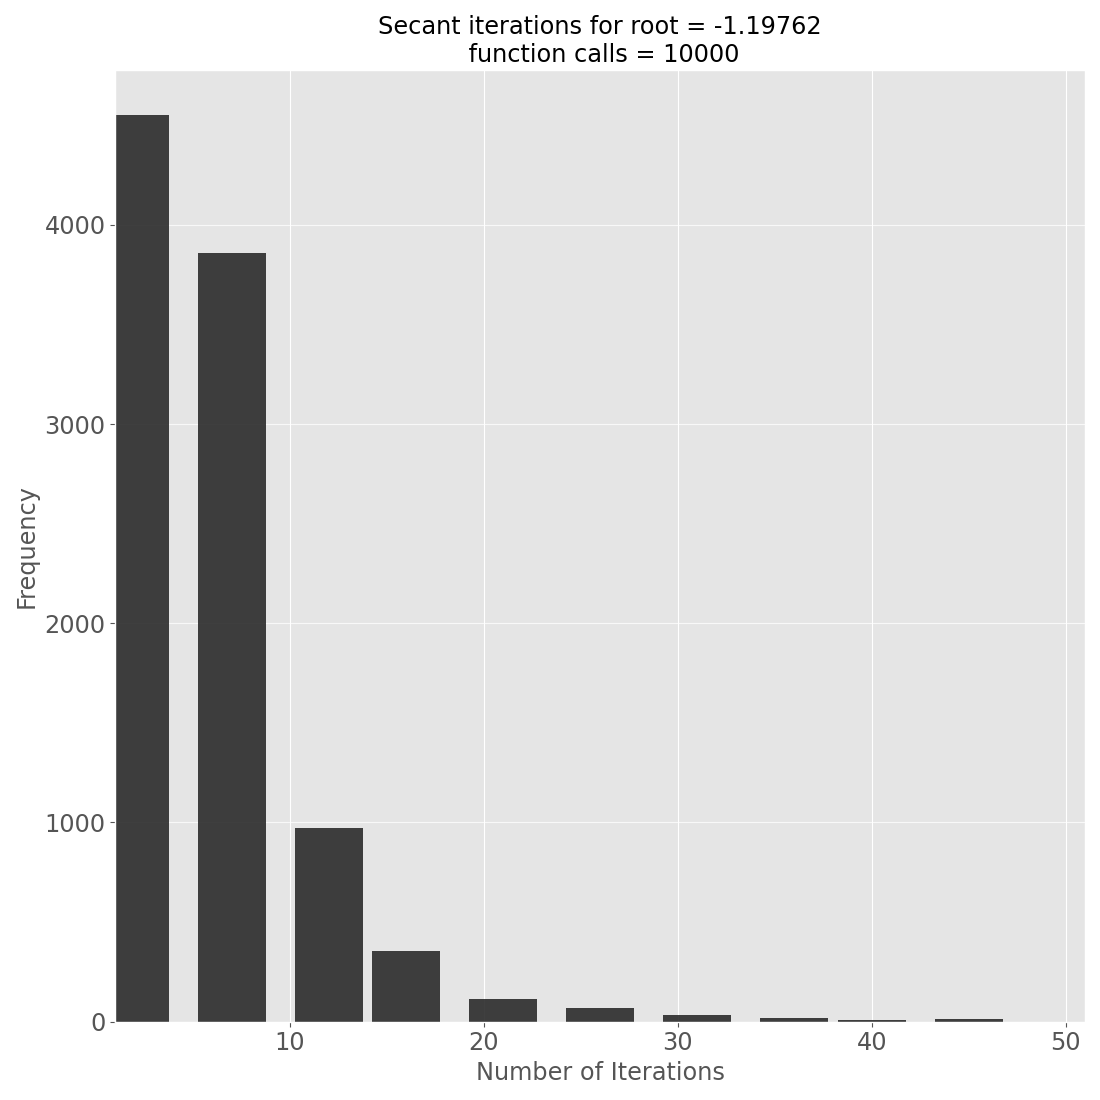
\includegraphics[scale=0.19]{secant_iterations_first_root.png} }}
    \quad
    \subfloat{{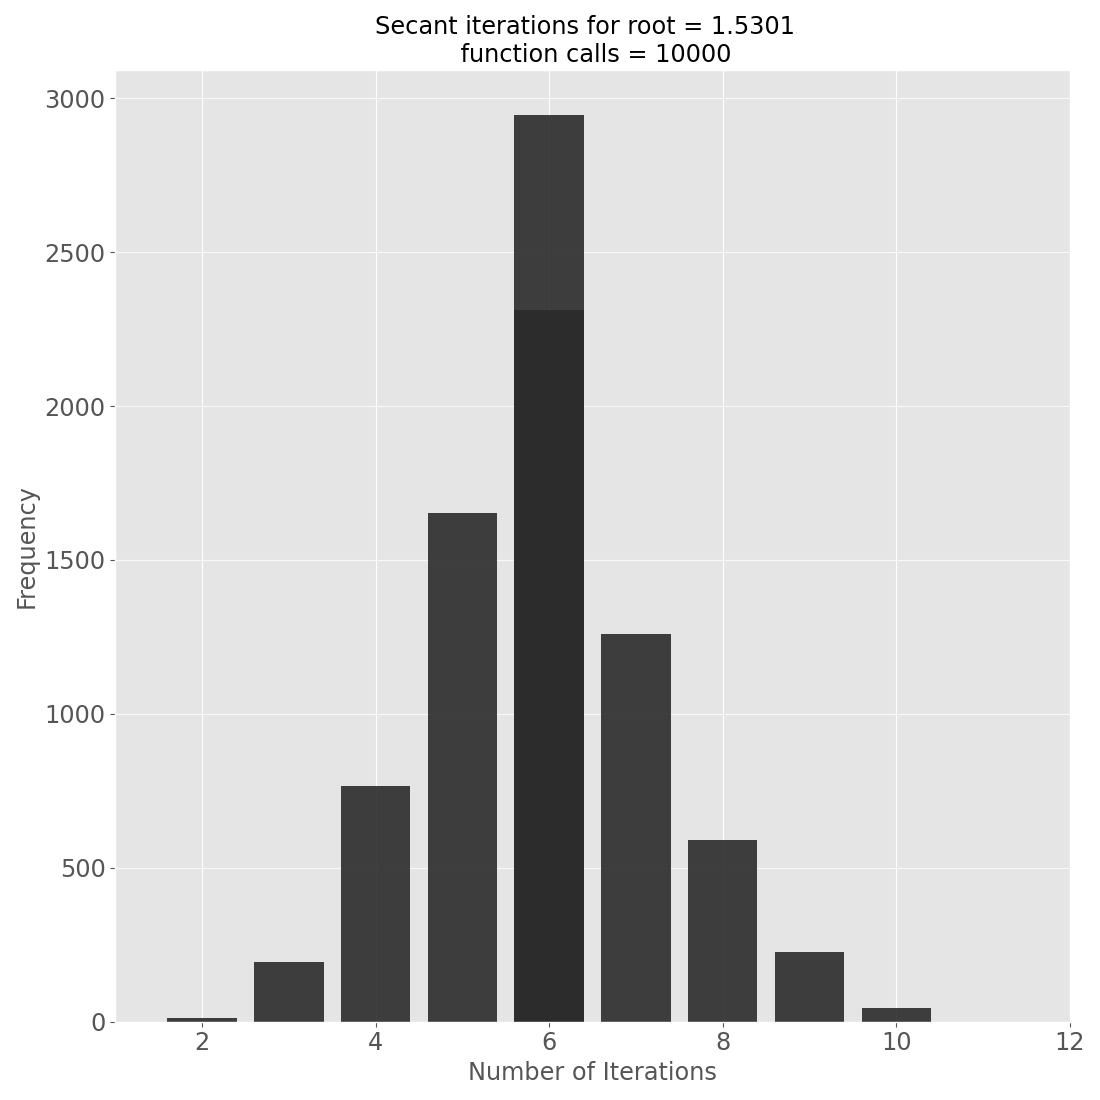
\includegraphics[scale=0.19]{secant_iterations_third_root.png} }}
    \caption{ Ιστογράμματα συχνοτήτων του αριθμού των επαναλήψεων για την μέθοδο της τέμνουσας. }
\end{figure}
Όπως παρατηρούμε από τα ιστογράμματα στο \textit{Σχήμα 26} η μέθοδος της τέμνουσας αποδίδει κυρίως σε αριθμούς επαναλήψεων κάτω από 10, με τις
περισσότερες απ' αυτές να είναι γύρω από το 6, αλλά σε κάποιες περιπτώσεις ( περίπου \textbf{20\%} του δείγματος ) ξεπερνάει τις 10.

\textbf{Συμπερασματικά}, έχουμε σύμφωνα με το δείγμα ότι έφοσον πληρούνται οι αντίστοιχες προϋποθέσεις για όλες τις μεθόδους η αποδοτικότερη και πιο σταθερή
στην απόδοση της από τις μεθόδους ως προς τον αριθμό των επαναλήψεων είναι η μέθοδος \textlatin{\textbf{Newton-Raphson}}. Στην συνέχεια, λιγότερο αποδοτικότερη είναι η μέθοδος της \textbf{τέμνουσας}
ενώ τέλος την χειρότερη απόδοση έχει η μέθοδος της \textbf{διχοτόμησης}. Εξάλλου, η τάξη σύγκλισης της μεθόδου \textlatin{\textbf{Newton-Raphson}} είναι
\textbf{\textlatin{p} = 2}, της μεθόδου της \textbf{τέμνουσας} \textbf{\textlatin{p} $\approx$ 1.62} ενώ της μεθόδου της \textbf{διχοτόμησης} \textbf{\textlatin{p} = 1}, οπότε τα συμπεράσματα από τα 
ιστογράμματα αιτιολογούνται από τις τάξεις σύγκλισης της κάθε μεθόδου.
 \end{document}